%!TEX root = thesis.tex

\chapter{Spätmittelalter}
\label{chapter-konzept}

Dieses Kapitel beschreibt die Wandlungen im Spätmittelalter, die vor allem durch den Machtverlust hervorgerufen wurden.

\section{Heiliges römisches Reich deutscher Nation}

Die Reichsidee war auch noch im Spätmittelalter lebendig, als die Macht des Kaisertums bereits beträchtlich geschwunden war. Heinrich VII., den Dante fast schon panegyrisch lobte, knüpfte direkt daran an und betonte die Bedeutung des Imperiums als Universalmacht, auch im Sinne der christlichen Heilsgeschichte. Dabei bediente er sich auch des römischen Rechts (wie schon die Staufer über 100 Jahre zuvor). Das imperiale Selbstverständnis Heinrichs VII., seine Kaiseridee, rief allerdings auch den Widerstand Frankreichs und des Papstes hervor.
\begin{figure}[h]
\centering
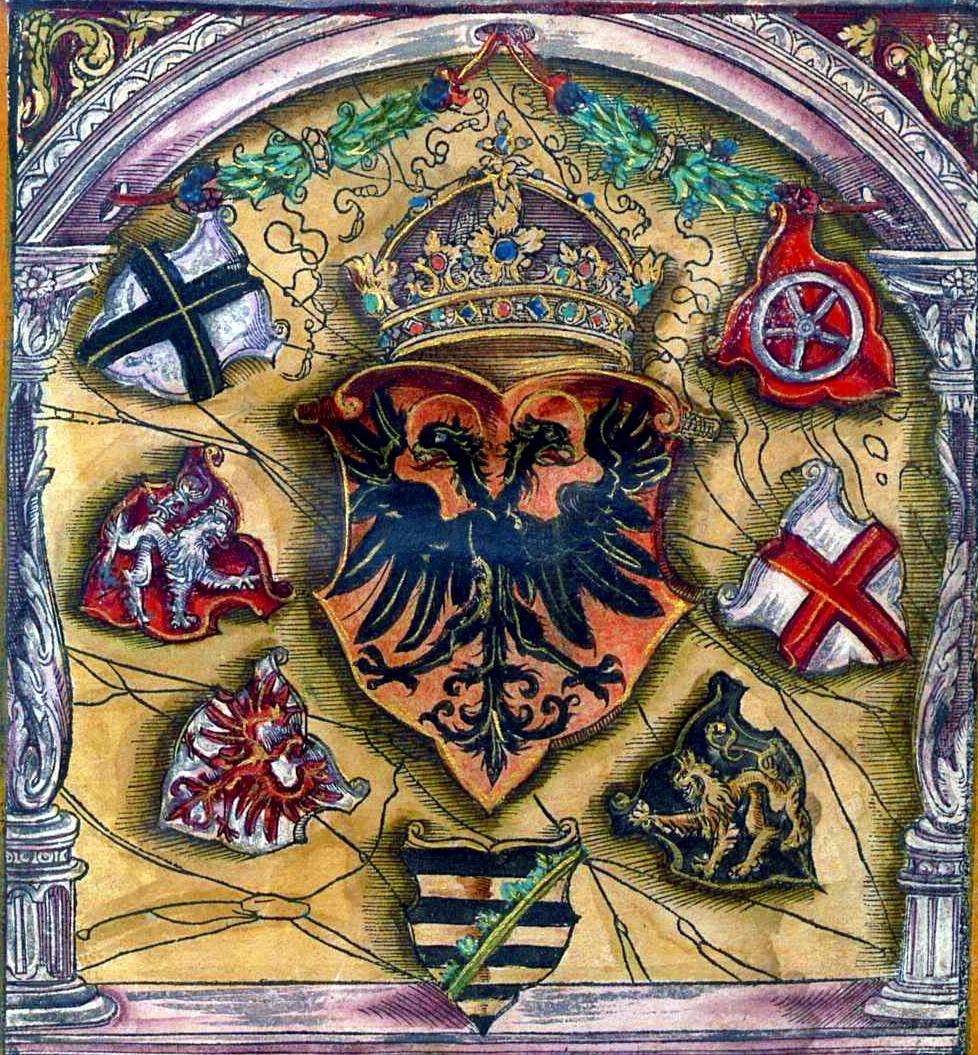
\includegraphics[width = 5cm, height= 7cm]{Kaiserwappen.jpg}
\caption{Wappen des Heiligen Römischen Reiches Deutscher Nation mit den Wappen der Kurfürsten. Fahnenbuch des Jacob Köbel (1545)}
\end{figure}
Der Zusatz „Deutscher Nation“ taucht in der Literatur erstmals 1438 auf, im Antrittsjahr von Albrecht II. 1486 wurde er erstmals in einem Gesetzestext erwähnt. Die Betonung des deutschen Charakters des Römischen Reiches verstärkte sich seit Ende des 15. Jahrhunderts, als die Macht des Kaisers in Reichsitalien de facto nicht mehr ins Gewicht fiel und sich im Wesentlichen auf das deutsche Herrschaftsgebiet beschränkte. Auch im Abwehrkampf gegen Karl den Kühnen von Burgund wurde diese Terminologie verwendet.


\section{Neue Legitimation}

Im Reich setzte sich mehr und mehr die Ansicht durch, dass der König (bzw. zukünftige Kaiser) von den Kurfürsten gewählt würde, der dann entweder vom Papst zum Kaiser gekrönt wurde oder – ab der Frühen Neuzeit – ohne Bestätigung durch den Papst in das Kaiseramt nachrückte. Das Papsttum hingegen hatte im Mittelalter immer darauf bestanden, dass es über die „Eignung“ des Kaisers selbst entscheiden könnte – was im Reich auf erheblichen Widerstand stieß (siehe Staufer). Der offizielle Königstitel bis zur Ottonenzeit lautete Rex Francorum („König der Franken“) im Regnum Francorum orientalium („Königreich der östlichen Franken“), danach Rex Romanorum („Römischer König“).

Nach der Kaiserkrönung wurde die Titulatur um den Zusatz semper Augustus ergänzt, der aber teilweise auch schon vor der Kaiserkrönung gebraucht wurde. Dieser Titel wurde als „allzeit Mehrer des Reiches“ verdeutscht, da man Augustus fälschlich vom lateinischen Verb augere („vermehren, vergrößern“) ableitete. Der Begriff Mehrer stand dabei für die Pflicht des Herrschers, die Rechte des Imperiums zu schützen und zu erhalten. Konkret bedeutete dies, dass der Kaiser die Entfremdung von Reichsrechten wie Regalien (wie in Italien) oder den Verlust von Gebieten (wie im westlichen Grenzraum an Frankreich) zu verhindern hatte.
\cite{Kintzinger}

